\documentclass[UTF8]{article}
\usepackage{graphicx}
\usepackage{subfigure}
\usepackage{amsmath}
\usepackage{makecell}
\usepackage[utf8]{inputenc}
\usepackage[space]{ctex} %中文包
\usepackage{listings} %放代码
\usepackage{xcolor} %代码着色宏包
\usepackage{CJK} %显示中文宏包
\usepackage{float}
\usepackage{makecell}
\usepackage{diagbox}
\usepackage{bm}
\usepackage{ulem} 
\usepackage{caption}
\usepackage{amssymb}
\usepackage{soul}
\usepackage{color}
\usepackage{geometry}
\usepackage{fancybox} %花里胡哨的盒子
\usepackage{xhfill} %填充包, 可画分割线 https://www.latexstudio.net/archives/8245
\usepackage{multicol} %多栏包
\usepackage{enumerate} %可以方便地自定义枚举标题
\usepackage{multirow} %表格中多行单元格合并
\usepackage{wasysym} %可以使用wasysym里的一堆奇奇怪怪的符号

\geometry{left = 1cm, right = 1cm, top=2cm, bottom=2cm}

\definecolor{mygreen}{rgb}{0,0.6,0}
\definecolor{mygray}{rgb}{0.5,0.5,0.5}
\definecolor{mymauve}{rgb}{0.58,0,0.82}
\lstset{
	backgroundcolor=\color{gray}, 
	%\tiny < \scriptsize < \footnotesize < \small < \normalsize < \large < \Large < \LARGE < \huge < \Huge
	basicstyle = \footnotesize,       
	breakatwhitespace = false,        
	breaklines = true,                 
	captionpos = b,                    
	commentstyle = \color{mygreen}\bfseries,
	extendedchars = false,
	frame = shadowbox, 
	framerule=0.5pt,
	keepspaces=true,
	keywordstyle=\color{blue}\bfseries, % keyword style
	language = C++,                     % the language of code
	otherkeywords={string}, 
	numbers=left, 
	numbersep=5pt,
	numberstyle=\tiny\color{mygray},
	rulecolor=\color{black},         
	showspaces=false,  
	showstringspaces=false, 
	showtabs=false,    
	stepnumber=1,         
	stringstyle=\color{mymauve},        % string literal style
	tabsize=4,          
	title=\lstname           
}

%\sum\nolimits_{j=1}^{M}   上下标位于求和符号的水平右端,
%\sum\limits_{j=1}^{M}   上下标位于求和符号的上下处,
%\sum_{j=1}^{M}  对上下标位置没有设定,会随公式所处环境自动调整。

%%%%%%%%%%%%%画图包%%%%%%%%%%%%%
\usepackage{tikz}
%%%%%%%%%%%%%画图背景包%%%%%%%%%%%%%
\usetikzlibrary{backgrounds}

%%%%%%%%%%%%%在tikz中画一个顶点%%%%%%%%%%%%%
%%%%%%%%%%%%%#1:node名称%%%%%%%%%%%%%
%%%%%%%%%%%%%#2:位置%%%%%%%%%%%%%
%%%%%%%%%%%%%#3:标签%%%%%%%%%%%%%
\newcommand{\newVertex}[3]{\node[circle, draw=black, line width=1pt, scale=0.8] (#1) at #2{#3}}
%%%%%%%%%%%%%在tikz中画一条边%%%%%%%%%%%%%
\newcommand{\newEdge}[2]{\draw [black,very thick](#1)--(#2)}
%%%%%%%%%%%%%在tikz中放一个标签%%%%%%%%%%%%%
%%%%%%%%%%%%%#1:名称%%%%%%%%%%%%%
%%%%%%%%%%%%%#2:位置%%%%%%%%%%%%%
%%%%%%%%%%%%%#3:标签内容%%%%%%%%%%%%%
\newcommand{\newLabel}[3]{\node[line width=1pt] (#1) at #2{#3}}

%%%%%%%%%%%%%强制跳过一行%%%%%%%%%%%%%
\newcommand{\jumpline} {\hspace*{\fill} \\}
%%%%%%%%%%%%%强制跳过一段%%%%%%%%%%%%%
\newcommand{\jumppar} {\hspace*{\fill} \par}
%%%%%%%%%%%%%关键点指令,可用itemise替代%%%%%%%%%%%%%
\newcommand{\average}[1]{\left\langle #1\right\rangle }
%%%%%%%%%%%%%表格内嵌套表格%%%%%%%%%%%%%
\newcommand{\keypoint}[2]{$\bullet$\textbf{#1}\quad#2\par}
%%%%%%%%%%%%%<T>平均值表示%%%%%%%%%%%%%
\newcommand{\tabincell}[2]{\begin{tabular}{@{}#1@{}}#2\end{tabular}}%放在导言区
%%%%%%%%%%%%%大黑点item头%%%%%%%%%%%%%
\newcommand{\itemblt}{\item[$\bullet$]}
%%%%%%%%%%%%%大圈item头%%%%%%%%%%%%%
\newcommand{\itemc}{\item[$\circ$]}
%%%%%%%%%%%%%大星星item头%%%%%%%%%%%%%
\newcommand{\itembs}{\item[$\bigstar$]}
%%%%%%%%%%%%%右▷item头%%%%%%%%%%%%%
\newcommand{\itemrhd}{\item[$\rhd$]}
%%%%%%%%%%%%%定义为%%%%%%%%%%%%%
\newcommand{\defas}{=_{df}}
%%%%%%%%%%%%%蕴含%%%%%%%%%%%%%
\newcommand{\imp}{\rightarrow}
%%%%%%%%%%%%%组合%%%%%%%%%%%%%
\newcommand{\comb}[2]{\left(\begin{array}{c}#1\\#2\end{array}\right)}
%%%%%%%%%%%%%exp%%%%%%%%%%%%%
\newcommand{\expo}[1]{\exp\left(#1\right)}

%%%%%%%%%%%%%双线分割线%%%%%%%%%%%%%
\newcommand*{\doublerule}{\hrule width \hsize height 1pt \kern 0.5mm \hrule width \hsize height 2pt}
%%%%%%%%%%%%%双线中间可加东西的分割线%%%%%%%%%%%%%
\newcommand\doublerulefill{\leavevmode\leaders\vbox{\hrule width .1pt\kern1pt\hrule}\hfill\kern0pt }
%%%%%%%%%%%%%左大括号%%%%%%%%%%%%%
\newcommand{\leftbig}[1]{\left\{\begin{array}{l}#1\end{array}\right.}
%%%%%%%%%%%%%矩阵%%%%%%%%%%%%%
\newcommand{\mat}[2]{\left[\begin{array}{#1}#2\end{array}\right]}
%%%%%%%%%%%%%可换行圆角文本框%%%%%%%%%%%%%

\newcommand{\ovalboxn}[1]{\ovalbox{\tabincell{l}{#1}}}
%%%%%%%%%%%%%设置section的counter, 使从0开始%%%%%%%%%%%%%
\setcounter{section}{0}




\begin{document}
\section{概率论基础}
\begin{itemize}
\item (蒲丰投针问题, 2020.2.25)桌面上画满间隔为$a$的平行线, 投长为$l(l < a)$的针, 求事件 $E=\{\mbox{针与某直线相交}\}$的概率.
\begin{figure}[H]
	\centering
	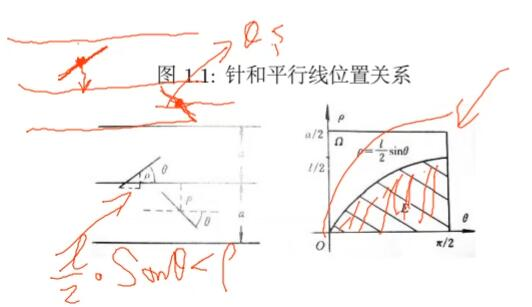
\includegraphics[scale=0.7]{pufengneedle.jpg}
	\caption{a}
\end{figure}\par

\item (Polya罐子模型, 2020.2.25)罐子中有a个白球b个黑球, 每次摸出一个后连同c个同色球放回. 证明第n次取球, 取出白球概率为$\frac{a}{a+b}$\\
\ovalboxn{
	假设第$n=k-1$次取, 概率为$\frac{a}{a+b}$, \\
	则有$P(A_k|A_1)=\frac{(a+c)}{(a+c)+b},\quad P(A_k|\overline{A_1})=\frac{(a)}{a+(b+c)}$,\\
	(实际上是假设最开始有a+c个白球, b个黑球, 这样$P(A_k))$当然就是$\frac{(a+c)}{(a+c)+b}$了)\\
	因此$P(A_k)=P(A_1)P(A_k|A_1)+P(\overline{A_1})P(A_k|\overline{A_1})=\frac{a}{a+b}$
}

\end{itemize}


\begin{figure}[H]
	\centering
	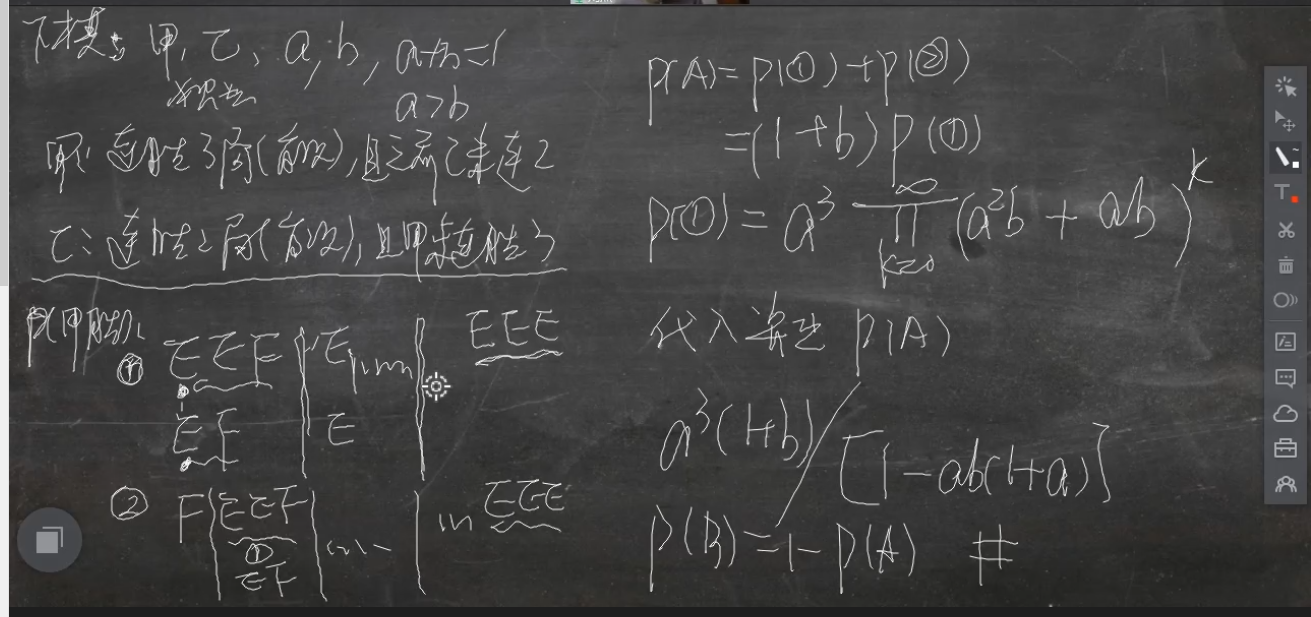
\includegraphics[scale=0.4]{2020_3_3_1.png}
\end{figure}\par

\section{随机变量及其分布}
\begin{itemize}
\item 离散\\
\begin{tabular}{|c|c|c|c|c|c|}
\hline
分布 & 标记 & 公式 & 均值 & 方差 & 特点\\
\hline
0-1分布 &  & $P(X=1)=p, P(X=0)=1-p$ & p & 0 & \\
\hline
伯努利分布 & $Ber(p)$ &  & $p$ & $p(1-p)$ & \\
\hline
二项分布 & $B(n,p)$ & $P(X=k)=\comb{n}{k}p^k(1-p)^{n-k}$ & $np$ & $np(1-p)$ & \tabincell{c}{极限是泊松分布\\再生性}\\
\hline
几何分布 & $G(p)$ & $P(X=k)=(1-p)^{k-1}p$ & $\frac{1}{p}$ & $\frac{q}{p^2}$ & \tabincell{c}{无记忆性} \\
\hline
Poisson分布 & $P(\lambda)$ & $P(X=k)=\frac{\lambda^k}{k!}e^{-\lambda},\lambda>0$ & $\lambda$ & $\lambda$ & 再生性 \\
\hline
离散均匀分布 & $U{a_1,a_2,\cdots,a_n}$ & & & & \\
\hline
\end{tabular}

\item 连续\\
\begin{tabular}{|c|c|c|c|c|c|}
\hline
分布 & 标记 & 公式 & 均值 & 方差 & 特点\\
\hline
正态分布 & $N(\mu, \sigma)$ & $f(x)=\frac{1}{\sqrt{2\pi}}\sigma\exp{-\frac{(x-\mu)^2}{2\sigma^2}}$ & $\mu$ & $\sigma^2$ & $aX+bY\sim N(a\mu_1+b\mu_2,a^2\sigma_1^2+b^2\sigma_2^2)$ \\
\hline
指数分布 & $Exp(\lambda)$ & $f(x)=\left\{\begin{array}{l}\lambda e^{-\lambda x}, x > 0\\0, x\le 0\end{array}\right.$ & $\frac{1}{\lambda}$ & $\frac{1}{\lambda^2}$ & 无记忆性 \\
\hline
Weibull分布 &  & $f(x)=\left\{\begin{array}{l}\lambda\alpha x^{\alpha-1} e^{-\lambda x^\alpha}, x > 0,\alpha>0\\0, x\le 0\end{array}\right.$ &  &  &  \\
\hline
均匀分布 &  & $f(x)=\left\{\begin{array}{l}\frac{1}{b-a}, a\le x\le b\\0, else\end{array}\right.$ & $\frac{a+b}{2}$ & $\frac{(b-a)^2}{12}$ &  \\
\hline
\end{tabular}

\item 多维\\
\begin{tabular}{|c|c|c|c|c|c|}
\hline
分布 & 标记 & 公式 & 均值 & 方差 & 特点\\
\hline
多项分布 &  & $P(X_1=k_1,\cdots,X_n=k_n)=\frac{n!}{k_1!\cdots k_n!}p_1^k\cdots p_n^k$ &  &  & $(p_1+\cdots+p_n)^n=\frac{n!}{k_1!\cdots k_n!}p_1^k\cdots p_n^k$ \\
\hline
二元正态 & $N(\mu_1,\mu_2,\sigma_1^2,\sigma_2^2,\rho)$ & \tabincell{c}{$\frac{1}{(2\pi\sigma_1\sigma_2\sqrt{1-\rho^2})}$\\$\exp\left\{-\frac{1}{2(1-\rho^2)}\left(\frac{(x-\mu_1)^2}{\sigma_1^2}-\frac{2\rho(x-\mu_1)(y-\mu_2)}{\sigma_1\sigma_2}+\frac{(y-\mu_2)^2}{\sigma_2^2}\right)\right\}$} &  &  &  \\
\hline
\end{tabular}
\item $\Phi(x)$和$\phi(x)$表示$N(0,1)$的分布函数和密度函数
\item 指数函数通常用来描述失效率(无老化寿命分布), 即在$\Delta x$这段时间内, 失效概率恒为$\lambda$
\item 失效率函数$\frac{F'(x)}{1-F(x)}=\frac{P(x\le X\le x+\delta x|X>x)}{\delta x}$
\item 三大分布
	\begin{itemize}
	\item 卡方分布: $X\sim\chi_n^2$, $X=\sum\limits_{i=1}^nX_i^2$
		\begin{itemize}
		\item $EX=n$, $Var(X)=2n$
		\end{itemize}
	\item t分布: $T\sim t_n$, $T=\frac{X_1}{\sqrt{X_2/n}}$,$X_1\sim N(0,1)$, $X_2\sim\chi_n^2$
		\begin{itemize}
		\item $ET=0$当$n\ge2$, $Var(T)=\frac{n}{n-2}$当$n\ge3$
		\item 类似标准正态, n无穷时趋于标准正态
		\end{itemize}
	\item F分布: $F\sim F_{n,m}$, $X_1\sim\chi_n^2,X_2\sim\chi_m^2, F=\frac{X_1/n}{X_2/m}$
		\begin{itemize}
		\item 图像类似卡方分布
		\item 若$Z\sim F_{m,n}$, 则$\frac{1}{Z}\sim F_{n, m}$
		\item 若$T\sim t_n$, 则$T^2\sim F_{1,n}$
		\item $F_{m,n}(1-\alpha)=\frac{1}{F_{n,m}(\alpha)}$
		\end{itemize}
	\end{itemize}
\end{itemize}

\subsection{连续型随机变量的条件分布}
有
$$f_{X|Y}(x|y)=\frac{f(x,y)}{f_Y(y)}$$

\subsection{随机变量的函数的概率分布}
$y=g(x)$严格单调连续, 反函数唯一为$x=h(y)$, 且$h'(y)$存在且连续, 则$Y=g(x)$也是连续型随机变量, 有$$p(y)=f(h(y))|h'(y)|$$\\
多元的则乘上Jacobi行列式的绝对值即可.

\section{数字特征}
\subsection{期望}
\begin{itemize}
\item $E(aX+bY)=aE(X)+b(Y)$
\item 独立随机变量$E(XY)=E(X)E(Y)$
\item $Eg(X)=\left\{\begin{array}{c}
\sum g(a_i)p_i\\
\int_{-\infty}^{\infty}g(x)f(x)dx
\end{array}\right.$
\item $E(Y|X=x)=\left\{\begin{array}{c}
\sum a_ip_i\\
\int_{-\infty}^{\infty}yf(y|x)dy
\end{array}\right.$
\item 全期望公式: $E(E(Y|X))=E(g(X))=EY$
\item $p$分位数: $P(X\le\mu_p)\ge p$则$\mu_p$是随机变量$X$的p分位数
\end{itemize}
\subsection{方差}
\begin{itemize}
\item $Var(X)=E(X-EX)^2=\sigma^2=EX^2-(EX)^2$
\item 若X,Y不相关, 则$Var(aX+bY)=a^2Var(X)+b^2Var(Y)$
\item 标准化随机变量: $X^*=\frac{X-EX}{\sqrt{Var(X)}}, EX^*=0, Var(X^*)=1$
\end{itemize}
\subsection{矩(Moment)}
\begin{itemize}
\item 矩: $E[(X-c)^r]$
\item 原点矩: $c=0$, 即$EX^r$
\item 中心矩: $E[(X-EX)^r]$
\item 均值是一阶原点矩, 方差是二阶中心矩
\item k阶阶乘矩: $E[X(X-1)\cdots(X-k+1)]$
\end{itemize}
\subsection{协方差}
\begin{itemize}
\item $Cov(X,Y)=E(X-EX)(Y-EY)=EXY-EXEY	$
\item $Var(X+Y)=Var(X)+Var(Y)+2E(X-EX)(Y-EY)$
\item 独立则$Cov(X,Y)=0$
\item $Cov(a_1X_1+a_2X_2, b_1Y_1+b_2Y_2)=\sum\limits_{i=1}^{2}\sum\limits_{j=1}^{2}a_ib_jCov(X_i,Y_j)$
\item 二元正态分布$(X,Y)\sim N(a,b,\sigma_1^2, \sigma_2^2,\rho)$, 则协方差矩阵为$\left[\begin{array}{cc}\sigma_1^2 & \rho\sigma_1\sigma2\\\rho\sigma_1\sigma2 & \sigma_2^2\end{array}\right]$
\item $[Cov(X,Y)]^2\le\sigma_1^2\sigma_2^2=Var(X)Var(Y)$等号成立当且仅当$Y=aX+b$
\end{itemize}
\subsection{相关系数}
\begin{itemize}
\item $\rho_{X,Y}=\frac{Cov(X,Y)}{\sqrt{Var(X)Var(Y)}}\in[-1,1]$, 等号成立当且仅当$X,Y$之间存在严格线性关系, $\rho_{X,Y}$的正负与线性关系斜率正负相同
\item 衡量变量之间的线性强度
\item $\rho=0$时称$X,Y$不相关, 只表示无线性关系
\item $\xi,\eta$不相关$\Leftrightarrow Cov(\xi, \eta)=0 \Leftrightarrow E\xi\eta=E\xi E\eta \Leftrightarrow Var(\xi+\eta)=Var(\xi)+Var(\eta)$
\item 独立一定不相关, 不相关却不一定独立. 只在二元正态分布下, 独立$\Leftrightarrow$不相关
\end{itemize}

\section{大数定律和中心极限定理}
\subsection{大数定律}
\begin{itemize}
\item 弱大数定律: 对任何$\epsilon>0$, $\lim\limits_{n\rightarrow\infty}P(|\xi_n-\xi|\ge\epsilon)=0$
\item 独立同分布数列$\{X_n\}$服从大数定律, $\bar{X}=\frac{1}{n}\sum\limits_{k=1}^nX_k\stackrel{P}{\longrightarrow}\mu$, $\mu$为$X_n$期望. 即依概率收敛到$X_n$的期望$\mu$
\item \textcolor{blue}{Markov不等式: $Y$非负, $\forall\epsilon>0, P(Y\ge\epsilon)\le\frac{EY}{\epsilon}$}
\item \textcolor{blue}{切比雪夫不等式: $P(|X-EX|\ge\epsilon)\le\frac{Var(X)}{\epsilon^2}$}
\end{itemize}
\subsection{中心极限定理}
\begin{itemize}
\item $\{X_n\}$独立同分布, 期望方差为$\mu,\sigma^2$, 则$\sum\limits_{i=1}^{n}X_i$的标准化形式$\frac{\sum\limits_{i=1}^{n}X_i-n\mu}{\sqrt{n}\sigma}$满足中心极限定理: $\lim\limits_{n\rightarrow\infty}F_n(x)=\Psi(x)$, $F_n(x)$为标准化形式的分布函数. 即$\frac{\sum\limits_{i=1}^{n}X_i-n\mu}{\sqrt{n}\sigma}\stackrel{d}{\longrightarrow}N(0,1)$(依分布收敛)
\end{itemize}

\section{数理统计的基本概念}
\subsection{常用统计量}
\begin{itemize}
\item 样本均值: $\bar{X}=\frac{1}{n}\sum\limits_{i=1}^nX_i$
\item 样本方差:$S^2=\frac{1}{n-1}\sum\limits_{i=1}^n(X_i-\bar{X})^2$
\item 样本原点矩: $a_k=\frac{1}{n}\sum\limits_{i=1}^nX_i^k$
\item 样本中心矩: $m_k=\frac{1}{n}\sum\limits_{i=1}^n(X_i-\bar{X})^k$. 如$\frac{n-1}{n}S^2=m_2$
\item 次序统计量: 排好序的$X_1\le X_2\le\cdots\le X_n$, 则$(X_1, X_2,\cdots, X_n)$称为次序统计量
	\begin{itemize}
	\item 样本中位数: $m_{\frac{1}{2}}=\left\{\begin{array}{ll}
	X_{(\frac{n+1}{2})}&\mbox{n is odd}\\
	\frac{1}{2}\left[X_{(\frac{n}{2})}+X_{(\frac{n}{2}+1)}\right]&\mbox{n is even}
	\end{array}\right.$
	\item 极值
	\end{itemize}
\item 经验分布函数
\end{itemize}
\subsection{重要定理}
\begin{enumerate}
\item 定理1: ${X_i}\ i.i.d.\sim N(a, \sigma^2)$, $X=\frac{1}{n}\sum\limits_{i=1}^nX_i$和$S^2=\frac{1}{n-1}\sum\limits_{i=1}^n(X_i-\bar{X})^2$分别为样本均值和样本方差, 则有
	\begin{enumerate}
	\item $\bar{X}\sim N(a,\frac{1}{n}\sigma^2)$
	\item $(n-1)S^2/\sigma^2\sim\chi_{n-1}^2$
	\item $\bar{X}$和$S^2$独立
	\end{enumerate}
\item ${X_i}\ i.i.d.\sim N(a, \sigma^2)$, $$T=\frac{\sqrt{n}(\bar{X}-a)}{S}\sim t_{n-1}$$
\item ${X_i}\ i.i.d.\sim N(a_1, \sigma_1^2)$, ${Y_i}\ i.i.d.\sim N(a_2, \sigma_2^2)$, 且$\sigma_1^2=\sigma_2^2=\sigma^2$, 相互独立. 则
$$T=\frac{(\bar{X}-\bar{Y})-(a_1-a_2)}{S_\omega}\sqrt{\frac{mn}{m+n}}\sim t_{n+m-2}$$
这里$(n+m-2)S_\omega=(m-1)S_1^2+(n-1)S_2^2$. 将$(\bar{X}-\bar{Y})$标准化
\item ${X_i}\ i.i.d.\sim N(a_1, \sigma_1^2)$, ${Y_i}\ i.i.d.\sim N(a_2, \sigma_2^2)$,$$F=\frac{S_1^2/\sigma_1^2}{S_2^2/\sigma_2^2}\sim F_{m-1,n-1}$$
\item  ${X_i}\ i.i.d.\sim Exp(\lambda)$, 则$$2\lambda n\bar{X}=2\lambda\sum\limits_{i=1}^nX_i\sim\chi_{2n}^2$$
\item 三大分布
	\begin{itemize}
	\item 卡方分布: $X\sim\chi_n^2$, $X=\sum\limits_{i=1}^nX_i^2$
		\begin{itemize}
		\item $EX=n$, $Var(X)=2n$
		\end{itemize}
	\item t分布: $T\sim t_n$, $T=\frac{X_1}{\sqrt{X_2/n}}$,$X_1\sim N(0,1)$, $X_2\sim\chi_n^2$
		\begin{itemize}
		\item $ET=0$当$n\ge2$, $Var(T)=\frac{n}{n-2}$当$n\ge3$
		\item 类似标准正态, n无穷时趋于标准正态
		\end{itemize}
	\item F分布: $F\sim F_{n,m}$, $X_1\sim\chi_n^2,X_2\sim\chi_m^2, F=\frac{X_1/n}{X_2/m}$
		\begin{itemize}
		\item 图像类似卡方分布
		\item 若$Z\sim F_{m,n}$, 则$\frac{1}{Z}\sim F_{n, m}$
		\item 若$T\sim t_n$, 则$T^2\sim F_{1,n}$
		\item $F_{m,n}(1-\alpha)=\frac{1}{F_{n,m}(\alpha)}$
		\end{itemize}
	\end{itemize}
\end{enumerate}

\section{参数估计}
\subsection{点估计}
\subsubsection{矩估计}
\subsubsection{最大似然估计}
\subsubsection{点估计的优良准则}
\begin{itemize}
\item 弱相合估计: $\lim\limits_{n\rightarrow\infty}P_{\theta_1,\cdots,\theta_n}(\left|T(X_1,\cdots,X_n)-g(\theta_1,\cdots, \theta_n)\right|\ge\epsilon)=0$
\item 无偏性: 设$\hat{g}(X_1,\cdots,X_n)$为待估计参数$g(\theta)$的一个估计量, 若$$E\hat{g}(X_1,\cdots,X_n)=g(\theta)$$则称$\hat{g}(X_1,\cdots,X_n)$为$g(\theta)$的\textbf{无偏估计量}
\item 相对有效性: 比较两个估计的方差, 小的更有效
\end{itemize}
\subsection{区间估计}
\subsubsection{枢轴变量法}
\begin{enumerate}
	\item 单正态总体. $X_1, X_2, \cdots, X_n i.i.d. N(\mu, \sigma^2)$
	\begin{itemize}
		\item 估计$\mu$, 未知$\sigma$
		$$\frac{\sqrt{n}(\overline{X}-\mu)}{S}\sim t_{n-1}$$
		
		\item 估计$\sigma$, 未知$\mu$
		$$\frac{(n-1)S^2}{\sigma^2}\sim \chi_{n-1}^2$$
		
		\item 估计$\sigma$, 已知$\mu=\mu_0$.\\
		$$\sum\limits_{i=0}^n\frac{(X_i-\mu_0)^2}{\sigma^2} \sim \chi_{n}^2$$
		
		\item 估计$\mu$, 已知$\sigma=\sigma_0$
		由$\overline{X}\sim N(\mu,\frac{1}{n}\sigma_0^2)$
		有$$\frac{\overline{X}-\mu}{\sqrt{\frac{1}{n}\sigma_0^2}} \sim N(0, 1)$$
					
	\end{itemize}
	
	\item 二正态总体. $X_1, X_2, \cdots, X_m i.i.d. N(\mu_1, \sigma_1^2)$, $Y_1, Y_2, \cdots, Y_n i.i.d. N(\mu_2, \sigma_2^2)$, \textbf{两组样本之间相互独立}
	\begin{itemize}
		\item 估计$\mu_1-\mu_2$, 未知$\sigma_1, \sigma_2$. \\
		根据$(\overline{X}-\overline{Y}) \sim N(\mu_1-\mu_2, \frac{1}{n}\sigma_1^2+\frac{1}{m}\sigma_2^2)$有
		$$\frac{(\overline{X}-\overline{Y})-(\mu_1-\mu_2)}{S_\omega\sqrt{\frac{m+n}{mn}}} \sim t_{n+m-2}$$
		这里$S_\omega=\frac{1}{m+n-2}(\sum\limits_{i=0}^{m}(X_i-\overline{X})^2+\sum\limits_{i=0}^{n}(Y_i-\overline{Y}))^2$
		
		\item 估计$\frac{\sigma_1}{\sigma_2}$, 未知$\mu_1, \mu_2$.\\
		根据$\frac{(n-1)S_1^2}{\sigma_1^2} \sim \chi_{n-1}^2$
		$$\frac{S_1^2}{S_2^2}\frac{\sigma_2^2}{\sigma_1^2} \sim F_{n-1, m-1}$$
		这里计算时注意$F_{n-1, m-1}(1-\frac{\alpha}{2})=1/F_{m-1, n-1}(\frac{\alpha}{2})$
		
		\item 估计$\mu_1-\mu_2$, 已知$\sigma_1=\sigma_2=\sigma_0$.
		根据$(\overline{X}-\overline{Y}) \sim N(\mu_1-\mu_2, \frac{1}{n}\sigma_1^2+\frac{1}{m}\sigma_2^2)$有
		$$\frac{(\overline{X}-\overline{Y})-(\mu_1-\mu_2)}{\sigma_0\sqrt{\frac{m+n}{mn}}} \sim N(0, 1)$$
						
		\item 估计$\frac{\sigma_1}{\sigma_2}$, 已知$\mu_1, \mu_2$.\\
		根据$\sum\limits_{i=0}^n\frac{(X_i-\mu_1)^2}{\sigma_1^2} \sim \chi_{n}^2$及$\sum\limits_{i=0}^m\frac{(Y_i-\mu_2)^2}{\sigma_2^2} \sim \chi_{m}^2$有
		$$\frac{\frac{1}{n}\sum\limits_{i=0}^n(X_i-\mu_1)^2}{\frac{1}{m}\sum\limits_{i=0}^m(Y_i-\mu_2)^2}\cdot\frac{\sigma_2^2}{\sigma_1^2} \sim F_{n, m}$$
		这里计算时注意$F_{n, m}(1-\frac{\alpha}{2})=1/F_{m, n}(\frac{\alpha}{2})$
		
	\end{itemize}
\end{enumerate}
\subsubsection{大样本法}
利用中心极限定理即可

\section{假设检验}
\subsection{一样本正态总体}
\begin{figure}[H]
	\centering
	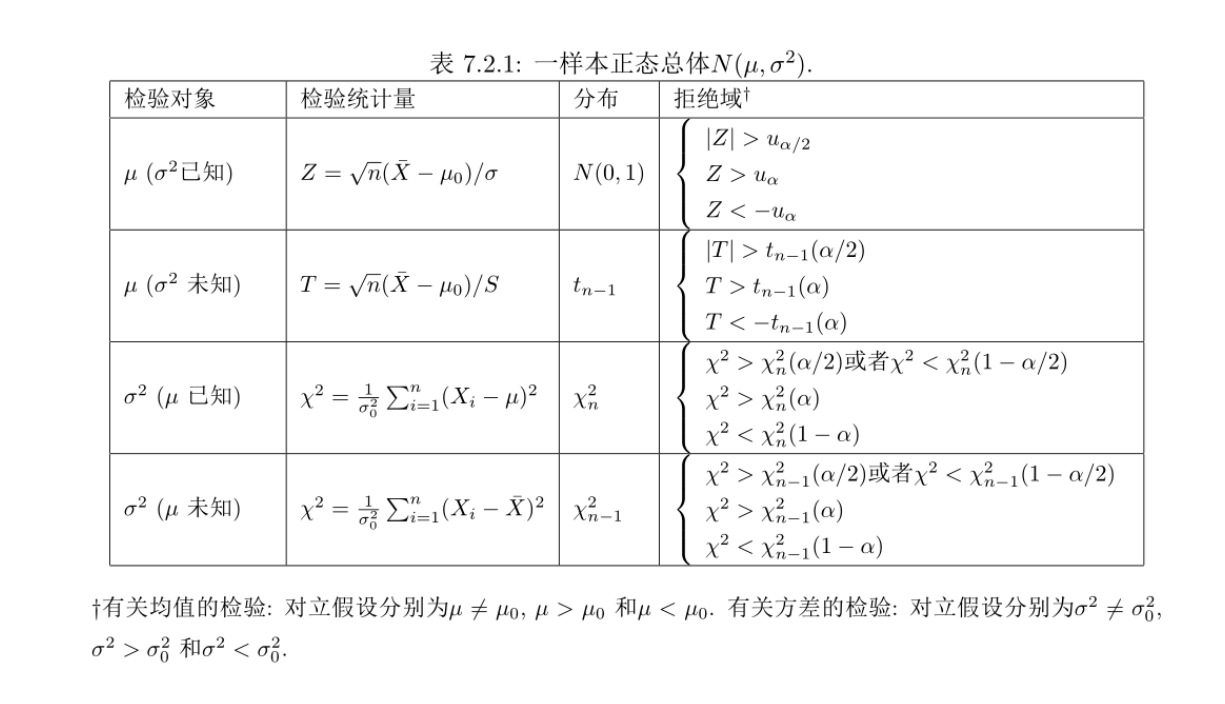
\includegraphics[width=\linewidth]{one_sample_norm.png}
\end{figure}
\subsection{两样本正态总体}
\begin{figure}[H]
	\centering
	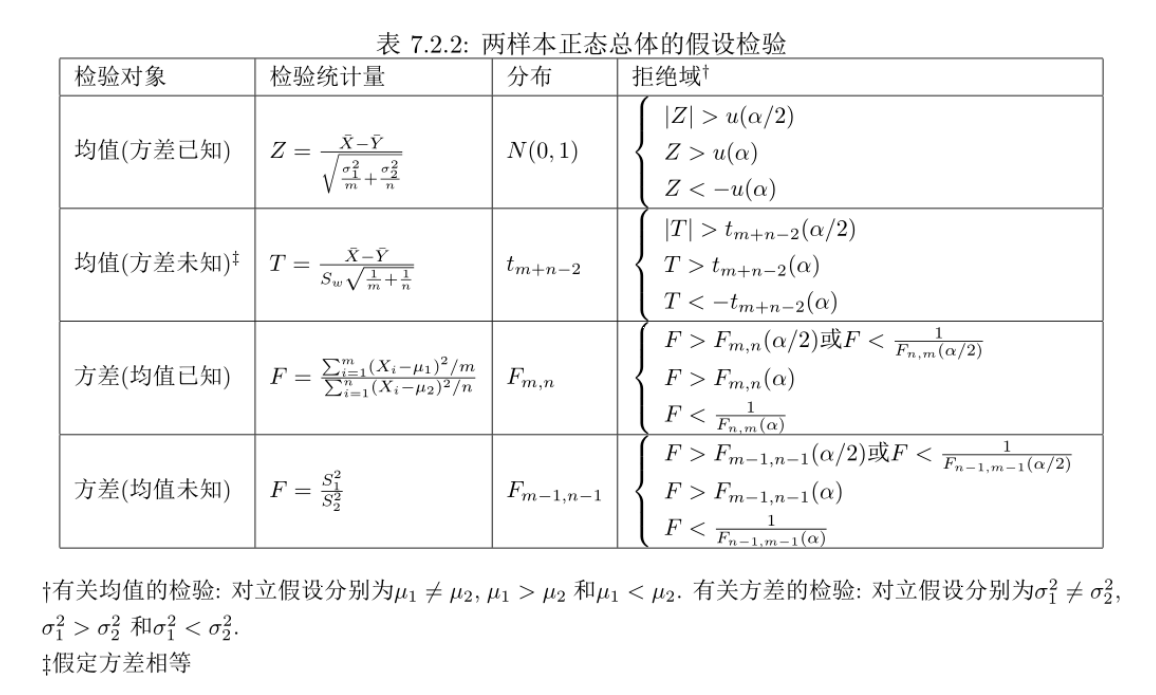
\includegraphics[width=\linewidth]{two_sample_norm.png}
\end{figure}
\subsection{成对数据}
作差构造一样本正态总体
\subsection{0-1分布参数$p$的检验}
由中心极限定理构造统计量$T=\sqrt{n}\frac{\bar{X}-p}{\sqrt{p_0(1-p_0)}}$

\subsection{拟合优度检验}
判断是不是来自某个分布. $H_0$: $X$服从分布$F$. 一般不必再写一个对立假设.\par
用Pearson提出的卡方拟合优度检验.
\subsubsection{离散}
理论频数和实际观测频数. 用
$$T=\sum\limits_{i=1}^k\frac{(n_i-np_i)^2}{np_i}\sim\chi_{k-1}^2$$
这里是将统计量$n_i$分布看成泊松分布, 均值方差都为$np_i$, 再由中心极限定理得到的, 其平方求和则为卡方分布. 但$\sum\limits_{i=1}^k n_i=k$, 因此自由度应该是$k-1$.\par
拒绝域: $T>\chi_{k-1}^2(\alpha)$\par
若含有r个未知参数, 要用最大似然估计代替这些参数, 则得到统计量
$$T=\sum\limits_{i=1}^k\frac{(n_i-n\hat{p}_i)^2}{n\hat{p}_i}\sim \chi_{k-1-r}^2$$
\subsubsection{列联表的独立性和齐一性检验}
\begin{itemize}
\item 独立性: $H_0$: 属性A与属性B独立. 用列联表.
\item 齐一性: 检验生存和死亡和住哪个医院无关. 转化为独立性. A的各个水平对应的B属性分布一致.
\end{itemize}

\subsubsection{连续}
分区间转化为离散型. 一般要求$n\hat{p}_i\ge5$, 如果不满足需要合并.


\end{document}



















